\section{Theoretical algorithms: guarantees and obstructions}
\label{sec:theory}

\subsection{Worst-case algorithms are exponential, but better than enumeration}
For $k\ge3$, arbitrary $k$-SAT is NP-complete. This is a worst-case fact;
it does not prove hardness of a particular random ensemble. No unconditional
exponential lower bound for every SAT algorithm is asserted here.
Table~\ref{tab:worstcase} lists useful theoretical benchmarks.
$O^*(\cdot)$ suppresses polynomial factors in the input size for fixed $k$.

\begin{table}[htbp]
\centering\small
\begin{tabularx}{\linewidth}{@{}L{.23\linewidth}L{.29\linewidth}Y@{}}
\toprule
Method & Time benchmark & Guarantee and scope \\
\midrule
2-SAT implication graph & $O(n+m)$ & Exact decision and witness construction. \\
Enumeration & $O^*(2^n)$ & Exact for all CNFs. \\
Sch\"oning local search & $O^*((2-2/k)^n)$ & Randomized bounded-error decision; a found witness is exact. \\
PPSZ family & About $O^*(1.3071^n)$ for general $3$-SAT & Randomized worst-case upper bound; stronger details below. \\
Liu: deterministic & $O^*(1.32793^n)$ for $3$-SAT & Exact; branching combined with derandomized local search. \\
\bottomrule
\end{tabularx}
\caption{Theoretical running-time benchmarks, not practical runtime forecasts.
See \citet{liu2018,scheder2024} and the more recent preprint
\citet{jiang2026}. The $3$-SAT bases must not be applied unchanged to larger $k$.}
\label{tab:worstcase}
\end{table}

Sch\"oning's algorithm starts at a random assignment and repeatedly flips
a randomly selected variable of an unsatisfied clause. Its analysis gives a
lower bound on the probability of reaching a solution, which independent
restarts amplify. PPSZ instead visits variables in random order, applying
bounded logical inference when possible and guessing otherwise
\citep{scheder2024}. Its general-$k$ bounds improve on this classical
local-search benchmark. The inference strength and polynomial factors matter:
a slightly better exponential base need not produce a faster implementation.

The July 2026 preprint \citep[Corollary 1.2]{jiang2026} gives
$O^*(1.307031578^n)$ for \emph{general} $3$-SAT by repeated PPSZ runs.
Its smaller $1.306969598$ base in Theorem 1.1 assumes a \emph{unique}
satisfying assignment and is not the general-case bound. These are the
most recent explicit PPSZ bounds checked for this survey; the tiny numerical
improvement has little practical significance. The deterministic
$1.32793$ bound is the published benchmark of \citet{liu2018}.

For randomized search, stopping after a prescribed number of unsuccessful
runs gives a one-sided error decision procedure: UNSAT inputs never acquire
a false witness, but SAT inputs can be missed. It does not yield a proof of
UNSAT. This differs from a complete deterministic solver, and from a
randomized solver whose logical search remains complete when allowed to finish.

\subsection{Algorithms with guarantees for uniform random formulas}
For large $k$, the central positive result is Coja-Oghlan's \emph{Fix}
algorithm \citep[Theorem 1.1]{coja2010}. There is a sequence $\varepsilon_k\to0$
such that, at
\begin{equation}
 \alpha\le (1-\varepsilon_k)\frac{2^k\log k}{k},
 \label{eq:fix}
\end{equation}
Fix outputs a satisfying assignment whp and has polynomial running time
(the cited implementation bound is $O((n+m)^{3/2})$).
This is a constructive guarantee over random inputs. It is not a claim that
the displayed leading term is a reliable cutoff at $k=3$.

The satisfiability scale $2^k\log2$ is much larger than
$2^k\log k/k$. Their leading-term ratio is $\log k/(k\log2)\to0$.
Thus provable efficient search reaches a vanishing fraction of the
satisfiable density interval in the large-$k$ limit. This separation motivates
an algorithmic phase-transition picture, but does not prove that every
polynomial-time method must fail above the Fix scale.

\begin{figure}[htbp]
\centering
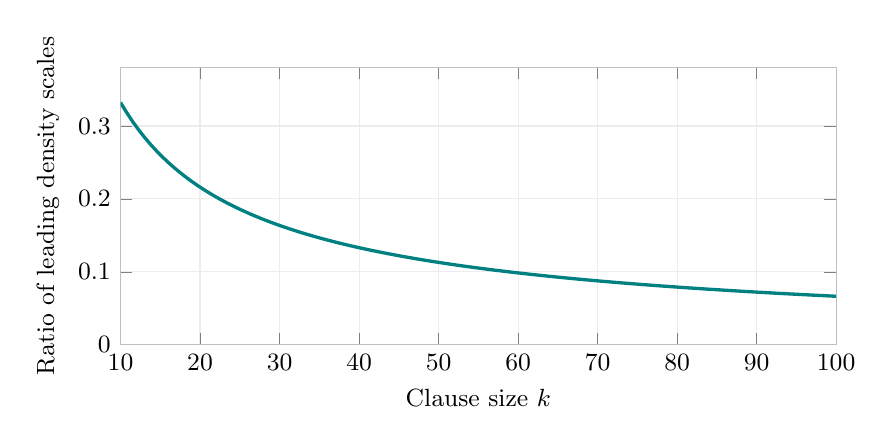
\begin{tikzpicture}
\begin{axis}[width=.88\linewidth,height=5.1cm,
 xmin=10,xmax=100,ymin=0,ymax=.38,
 xlabel={Clause size $k$},ylabel={Ratio of leading density scales},
 tick label style={font=\small},label style={font=\small},
 grid=major,grid style={gray!15},axis line style={gray!50},
 samples=120,domain=10:100]
\addplot[teal,very thick] {ln(x)/(x*ln(2))};
\end{axis}
\end{tikzpicture}
\caption{The analytic ratio $\log k/(k\log2)$. This compares the leading
large-$k$ expressions in \eqref{eq:fix} and \eqref{eq:largek}; it is not a
plot of measured algorithmic thresholds or a finite-$k$ guarantee.}
\label{fig:gap}
\end{figure}

Bresler and Huang prove obstructions for formally specified low-degree
polynomial and local algorithm classes at a constant multiple of this scale
\citep[Theorems 2.6 and 2.13]{bresler2021}. Their main low-degree theorem
uses $\alpha=\kappa2^k\log k/k$, $\kappa>\kappa_*\approx4.911$, and
sufficiently large $k$, with degree, normalization and success-probability
conditions. In particular, that theorem rules out a specified very high
success probability, not every nonzero success probability. The local-algorithm
result is stronger within its narrower class. Neither is a lower bound for
all polynomial-time algorithms, all CDCL implementations or finite-$k$ GPU
methods. The geometry of separated solution clusters and overlaps helps
explain these results; ``clustering implies hardness'' without a computational
model is only a heuristic.

\subsection{Proving UNSAT can be harder than predicting it}
At fixed density above the threshold, typical formulas are UNSAT. Efficiently
certifying this is a different question. A classical general polynomial-time
strong-refutation guarantee applies at
$m\ge\widetilde O(n^{k/2})$, with logarithmic factors and constants as in
\citet[Theorem 2.3 and Section 4]{allen2015}. For $3$-SAT this is about
$n^{3/2}$ clauses, much denser than the constant-density regime
$m\asymp4.27n$. It is a useful rigorous benchmark, not an efficient
near-threshold decision algorithm or a claim of optimality among all methods.

Resolution proof complexity supplies a concrete obstruction. Random $3$-CNF
formulas at suitable fixed UNSAT densities require exponential-size resolution
refutations whp; see \citet[Section 4.3]{ben2001}. This explains why
resolution-based search can struggle even when UNSAT is overwhelmingly
probable. The conclusion is specific to the proof system. Solvers with stronger
inference, extensions or inprocessing cannot all be identified with bare
resolution without checking the corresponding proof simulation.
